
\chapter{Materiais e Métodos}

\section{Datasets}

Bases de dados para treinamento ou teste de algoritmos de estimação de profundidade consistem em imagens RGB de uma cena e sua anotação correspondente em profundidade. Ao longo do tempo, diversos \textit{datasets} foram propostos para este fim com variações em formatos de anotações, tipos de cena (interior ou exterior), métodos de captura, qualidade, resolução e tamanho \textcolor{red}{colocar citações que tem na seção 3 do midas 1}.

Geralmente são empregados sensores e outras tecnologias como \textit{Stereo Matching} e \textit{Structure from Motion} para criar os \textit{datasets} de profundidade, porém, são abordagens muito complexas, custosas, ou inviáveis em algumas situações particulares, por exemplo, obter mapas de profundidades densos a partir de veículos em movimento  \cite{yang2024depthv1}.
Cada \textit{dataset} possui suas próprias características, problemas e viéses. Dados com informação de profundidade e em alta qualidade são complexos de adquirir, sendo que os melhores conjuntos são utilizados no treinamento dos modelos presentes na literatura \cite{ranftl2020towards}. 

Para avaliar os modelos de estimação de profundidade, será utilizado o protocolo de \textit{zero-shot cross-dataset transfer}, i.e. realizar os testes e métricas em bases de dados que não compuseram os conjuntos de treinamentos dos modelos analisados. A performance em \textit{cross-dataset} é considerada uma aproximação mais fiel da performance em mundo real em uma aplicação, pois os conjuntos de testes relativos aos conjuntos utilizados no treinamento podem refletir os mesmos viéses e situações \cite{ranftl2020towards}.

Dessa forma, para escolha das bases de dados a serem utilizadas para teste, temos os critérios: i) não ter composto o conjunto de treinamento dos modelos escolhidos para comparação, ii) conter dados válidos para avaliação considerando anotações precisas de profundidade, ou caso sejam esparsas, possuam máscara para indicar os pixels válidos, iii) ser uma base de dados conceituada na literatura. Os \textit{datasets} escolhidos e suas características podem ser visualizados na Tabela \ref{tabdata}.

% PESQUISA ANTIGA -------------------------------------------------------------------
% O presente trabalho exige um tipo de base de dados pouco encontrado na literatura, trios de imagem RGB, mapa de profundidade com erros e um outro mapa de profundidade denso e completo. De acordo com \cite{zhang2018deep}, uma das maneiras de se obter esses dados seria capturar imagens com uma câmera RGB-D de baixo custo e alinha-las com outra captura simultânea de um sensor mais preciso, porém essa abordagem é muito custosa, além de que não há disponibilidade de grandes conjuntos para treinamento.

% O presente projeto pretende utilizar como base de dados principal o \textbf{Hypersim}. Um \textit{dataset} para compreensão de cenas baseado em cenas sintéticas fotorrealistas. Contendo 77.400 imagens de 461 cenas \textit{indoor} com pares de RGB e mapas de profundidade calculado deterministicamente, além de outras informações como normais de superfície, rótulos de segmentação e detecção de objetos e entre outros \cite{roberts2021hypersim}.

% Please add the following required packages to your document preamble:
% \usepackage{graphicx}
\begin{table}[h]
    \centering
    \caption{Características dos datasets utilizados no trabalho}
    \label{tabdata}
    \resizebox{\textwidth}{!}{%
    \begin{tabular}{ccccccc}
    \hline
    \textbf{Dataset} & \textbf{Sensor} & \textbf{Anotação} & \textbf{Tipo} & \textbf{Cenário} & \textbf{Num. Imagens} & \textbf{Resolução} \\ \hline
    KITTI  & LiDAR         & Esparça & Real      & Outdoor        & 44 K   & 1024 $\times$ 320  \\
    Nyu-V2 & Kinect V1     & Densa   & Real      & Indoor         & 1449   & 640 $\times$ 480   \\
    DIODE  & Laser Scanner & Densa   & Real      & Indoor/Outdoor & 25,5 K & 768 $\times$ 1024  \\
    SINTEL & -             & Densa   & Sintético & Indoor/Outdoor & 1064   & 1024 $\times$ 436  \\
    ETH3D  & Laser Scanner & Densa   & Real      & Indoor/Outdoor & 454    & 6048 $\times$ 4032 \\ \hline
    \end{tabular}%
    }
    \end{table}


\subsection{NYUv2}


%% refazer o texto

O \textit{dataset} NYUv2 é um dos mais utilizados em tarefas de visão computacional que envolvam estimação de profundidade, segmentação de cenas e reconecimento de objetos. Possui 1449 pares de imagens RGB e mapas de profundidade densos em diversas cenas \textit{indoor} divididos em 795 para treinamento e 654 para teste \cite{silberman2012indoor}. A resolução das imagens é de 640 $\times$ 480 pixels. O equipamento de aquisição foi o equipamento Microsoft Kinect que utiliza a técnica de emissão de luz estruturada, que produz resultados precisos de informação de profundidade. Além dos pares RGB-D, também é disponibilizado os dados de leitura dos sensores puros em que é possível encontrar aproximadamente 70\% de pixels com informação válida de profundidade, no entanto, as imagens finais foram processadas utilizando um método de correção, resultando em um mapa denso, como observado na Figura \ref{exnyuv2}. Entre as cenas observadas no \textit{dataset}, podemos citar quartos, cozinhas, sala de aula, banheiro e etc. Além das informações de profundidade, a base de dados provém rótulos de segmentação de objetos e relações de suporte entre eles \cite{lahiri2024deep}.

\begin{figure}[h]
    \centering
    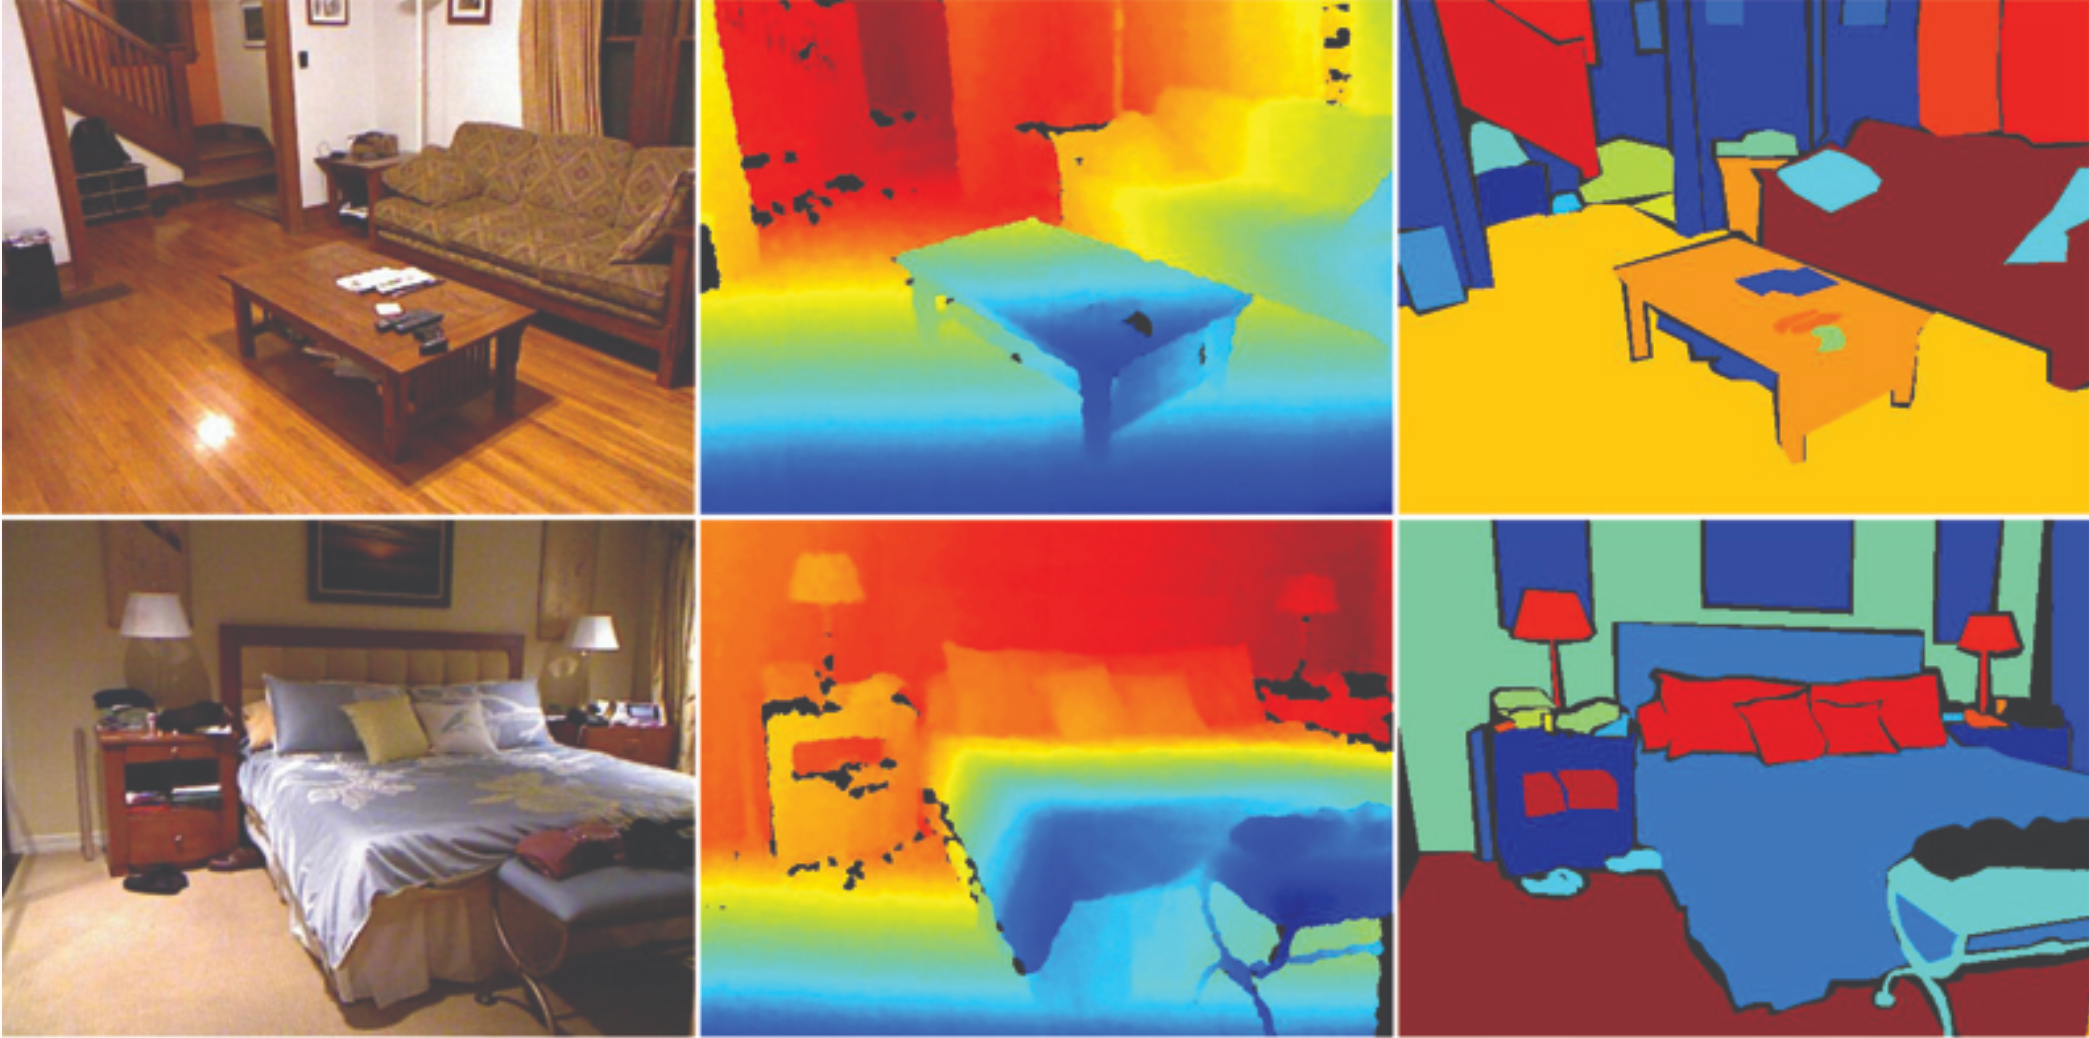
\includegraphics[width=\textwidth]{fig/example_nyu.png}
    \caption{Exemplo do dataset NYU Depth v2}
    \label{exnyuv2}
\end{figure}

\subsection{KITTI}



\subsection{SINTEL}

\subsection{ETH3D}

O ETH3D é uma base de dados geralmente utilizada para reconstrução em vistas múltiplas e \textit{stereo matching}. Contém dados de treinamento com imagens RGB \textit{multiview}, capturadas com câmeras DSLR e \textit{ground truth} de profundidade capturado utilizando um escâner a laser Faro Focus X 330. Oferece três versões de imagens de profundidade, uma correspondente à leitura bruta do sensor (\textit{raw}), outra com \textit{outliers} removidos por trabalho manual e uma ferramenta automática (\textit{clean}) e uma com \textit{outliers} e pontos observados por uma única imagem RGB removidos. A partição de teste não contém \textit{groundtruth}. A base de dados é associada à um desafio aberto ao público. Inclui cenas tanto internas quanto externas, oferecendo um protocolo de avaliação bem variado \cite{lahiri2024deep} \cite{schops2019bad}. 

\subsection{DIODE}

O \textit{dataset} DIODE (\textit{Dense Indoor and Outdoor Depth Dataset}), é uma base de dados para estimação monocular de profundidade e consiste em 8574+25 imagens de ambientes internos e 16.884+446 de ambientes externos para treinamento e teste. Possui resolução de 768 $\times$ 1024 com faixa de distâncias entre 50m e 300m para os ambientes internos e externos respectivamente. O equipamento de aquisição é o escâner a laser Faro Focus S350. Alguns exemplos do \textit{dataset} podem ser visualizados na Figura \ref{exdiode}.

\begin{figure}[h]
    \centering
    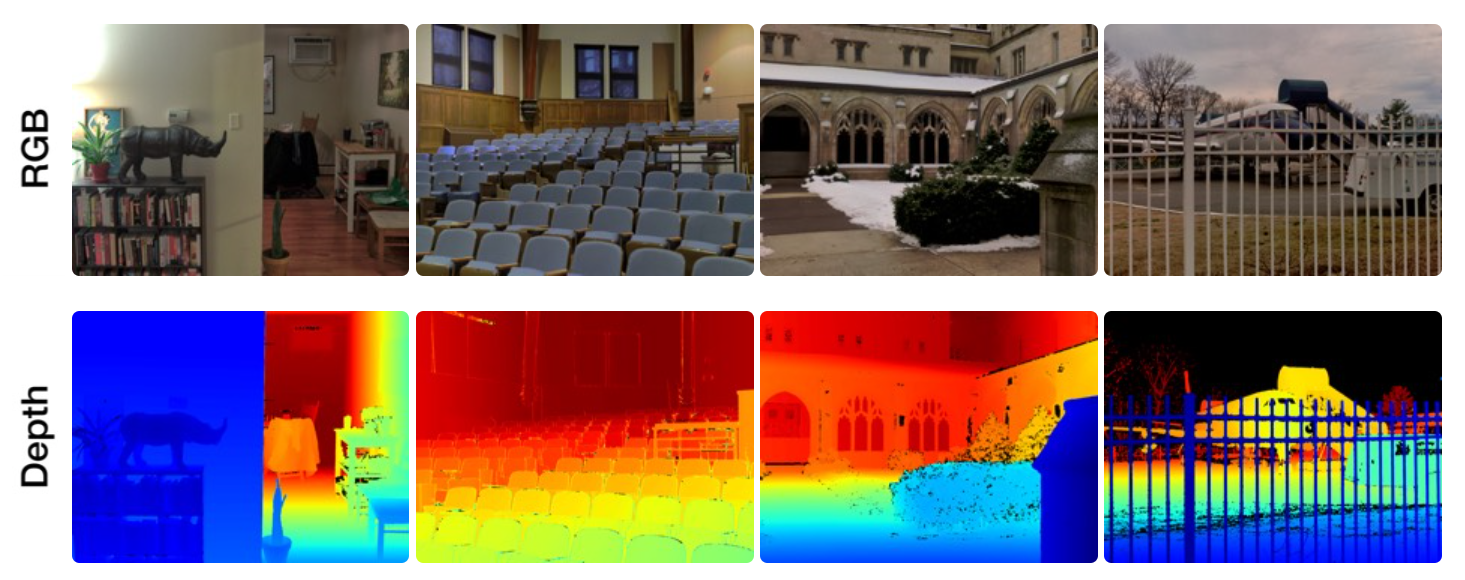
\includegraphics[width=\textwidth]{fig/example_diode.png}
    \caption{Exemplo do dataset DIODE}
    \label{exdiode}
\end{figure}

\section{Modelos Escolhidos}

\section{Protocolo de Avaliação}

\section{Método de Transformação de Intensidades (pós-processamento)}

Um mapa de profundidade inferido por um método de estimação de profundidade possui a característica de ser denso, pois todos os pixels possuem um valor predito associado, preciso, bem detalhado, de acordo com os últimos trabalhos do estado da arte porém é relativo, i.e. o valor de cada pixel é apenas correlacionado com a medição de distância real por um fator desconhecido. Já um mapa de profundidade adquirido com um sensor físico consegue representar as grandezas de forma métrica (em metros, centímetros ou até milimétros), mas pode ter características negativas associadas a depender do dispositivo de aquisição, podendo conter áreas falhas que não possuem medição associada, ou um elevado grau de esparsidade. O método de transformação de intensidades para transferência de domínio almeja como resultado uma imagem de profundidade que possuam as características positivas dos dois casos anteriormente citados. 

O método proposto por este trabalho consiste em uma transformação de intensidades que é projetada para cada imagem de um conjunto de dados utilizando pontos correspondentes em ambas e associando uma transformação linear para cada ponto, como visualizado na Figura \ref{posproc}. 


\begin{figure}[h]
    \centering
    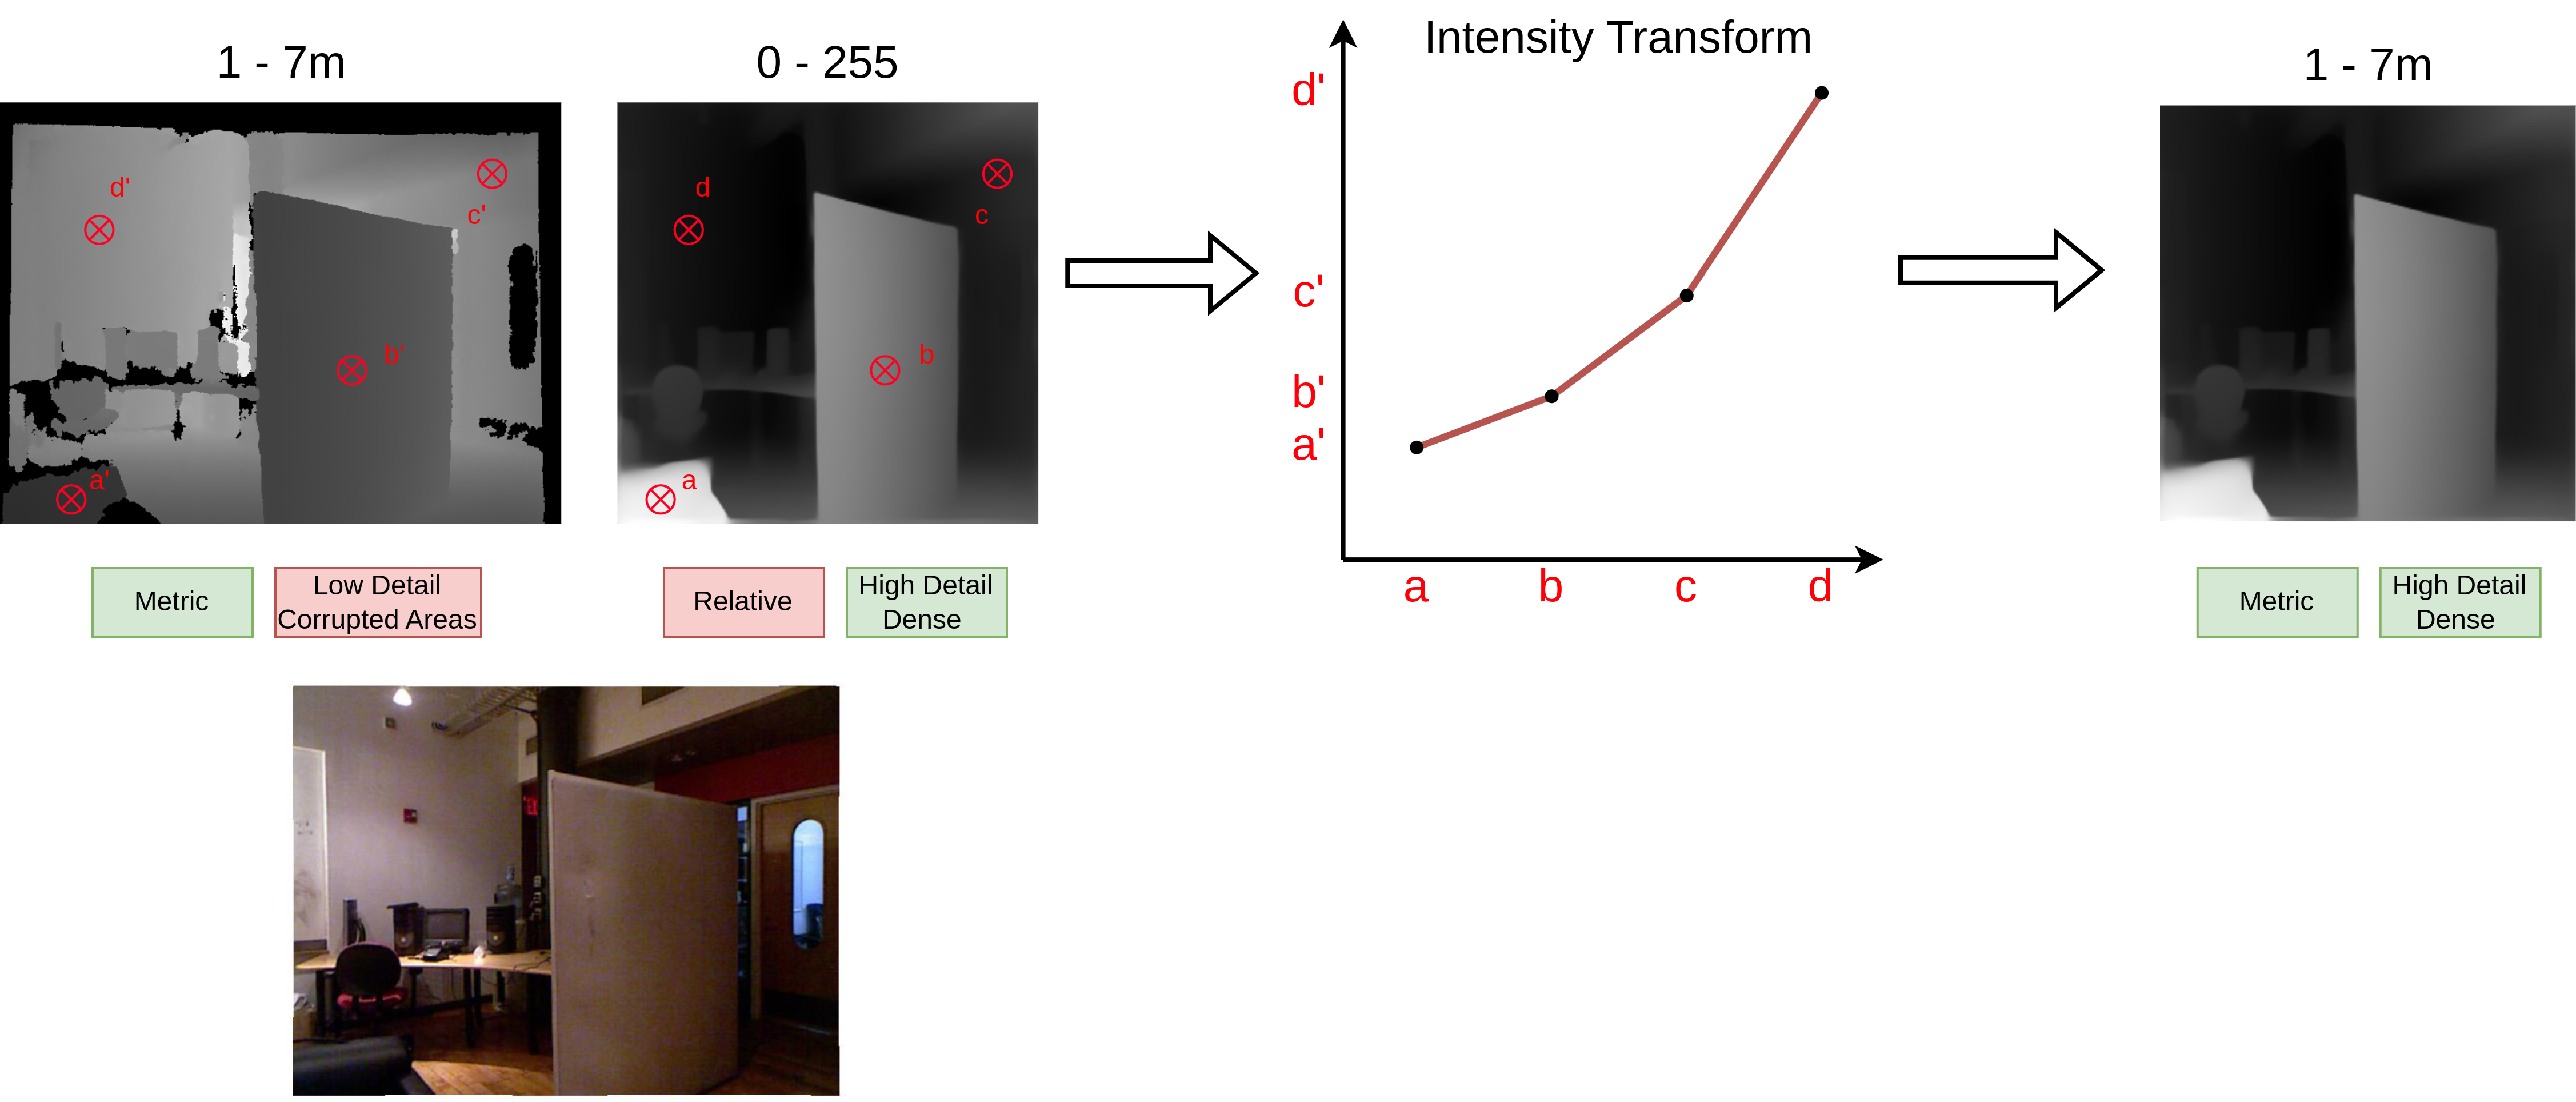
\includegraphics[width=\textwidth]{fig/diagram_normalization_white.png}
    \caption{Diagrama do método de transferência de domínio}
    \label{posproc}
\end{figure}

O método proposto diferencia-se do tradicional baseado em fator de escala e deslocamento por mínimos quadrados pois é associada uma função linear para cada região na quantização da imagem, o que propicia uma correção adaptada para cada proporção de distância. Ressalta-se que o método não será utilizado protocolo de avaliação dos modelos de estimação de profundidade, mas sim o que é mais prevalente na literatura.

Aos conjuntos de dados que possuem leituras métricas de sensores, será comparado o resultado da técnica de pós-processamento e o resultado de estimadores métricos de profundidade.

\section{Correção de mapas de profundidade} 

Para a tarefa de correção de mapas de profundidade utilizando redes neurais, o trabalho de \cite{hu2022deep} propôs duas categorias principais que se diferenciam pelos dados utilizados:

\begin{itemize}
    \item \textbf{Correção não-guiada} (Figura \ref{ung}): Objetiva completar diretamente as partes faltantes utilizando como entrada somente o mapa de profundidade.
    \item \textbf{Correção guiada} (Figura \ref{early} e \ref{late}): Objetiva completar as partes faltantes utilizando como entrada tanto o mapa de profundidade quanto a imagem RGB correspondente.
\end{itemize}

\begin{figure}[h]
    \centering
    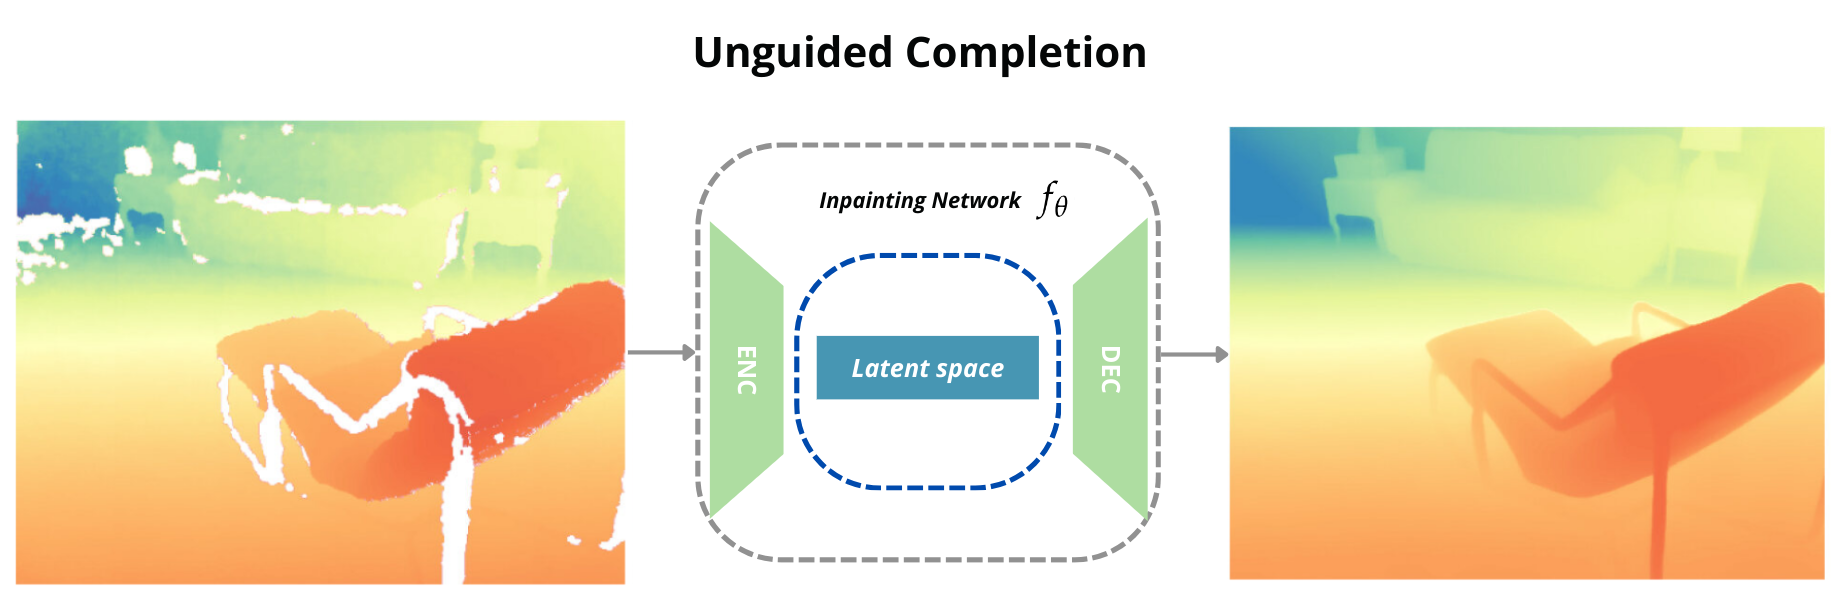
\includegraphics[width=\textwidth]{fig/unguided.png}
    \caption{Esquema de correção não-guiada.}
    \label{ung}
\end{figure}

A escolha da categoria de correção depende da quantidade de erros nas imagens. Quando há uma pequena quantidade de pixels inválidos, a correção não-guiada pode ser adequada, visto que não é necessário uma profunda extração de características dos dados. No entanto, no caso contrário, o uso de métodos guiados é indicado dado que existam grandes regiões com ausência de informação de profundidade ou que o mapa apresente uma grande esparsidade. Sendo necessário recorrer a extração dos atributos presentes na imagem RGB como bordas, contornos, estruturas de objetos não identificados pelo sensor e característica de descontinuidade de superfícies \cite{hu2022deep}.

Ainda no trabalho de \cite{hu2022deep}, nomeia-se outras subcategorias de técnicas de correção guiada. Uma delas é chamada de \textit{Early Fusion} (Figura \ref{early}) e consiste em utilizar a imagem RGB concatenada ao mapa de profundidade com erros como entrada da rede neural. Essa técnica possui a vantagem de ser simples e de baixa complexidade. A outra, conhecida como \textit{Late Fusion} (Figura \ref{late}) envolve transferir a fusão da imagem RGB com o mapa em ramos distintos da rede neural, chamados \textit{RGB Encoder-Decoder} e \textit{Depth Encoder-Decoder}.

\begin{figure}[h]
    \centering
    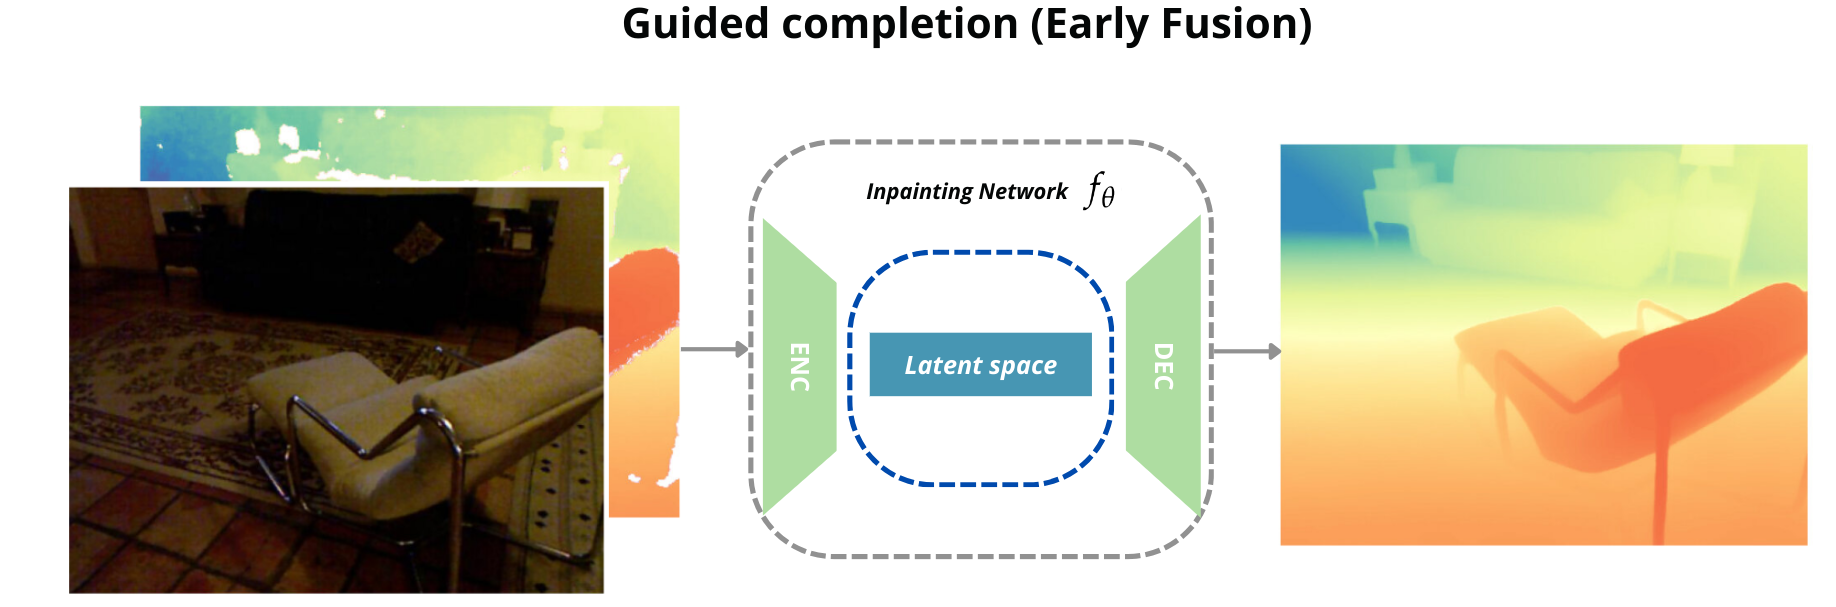
\includegraphics[width=\textwidth]{fig/earlyfusion.png}
    \caption{Esquema de correção guiada com \textit{Early Fusion}.}
    \label{early}
\end{figure}

\begin{figure}[h]
    \centering
    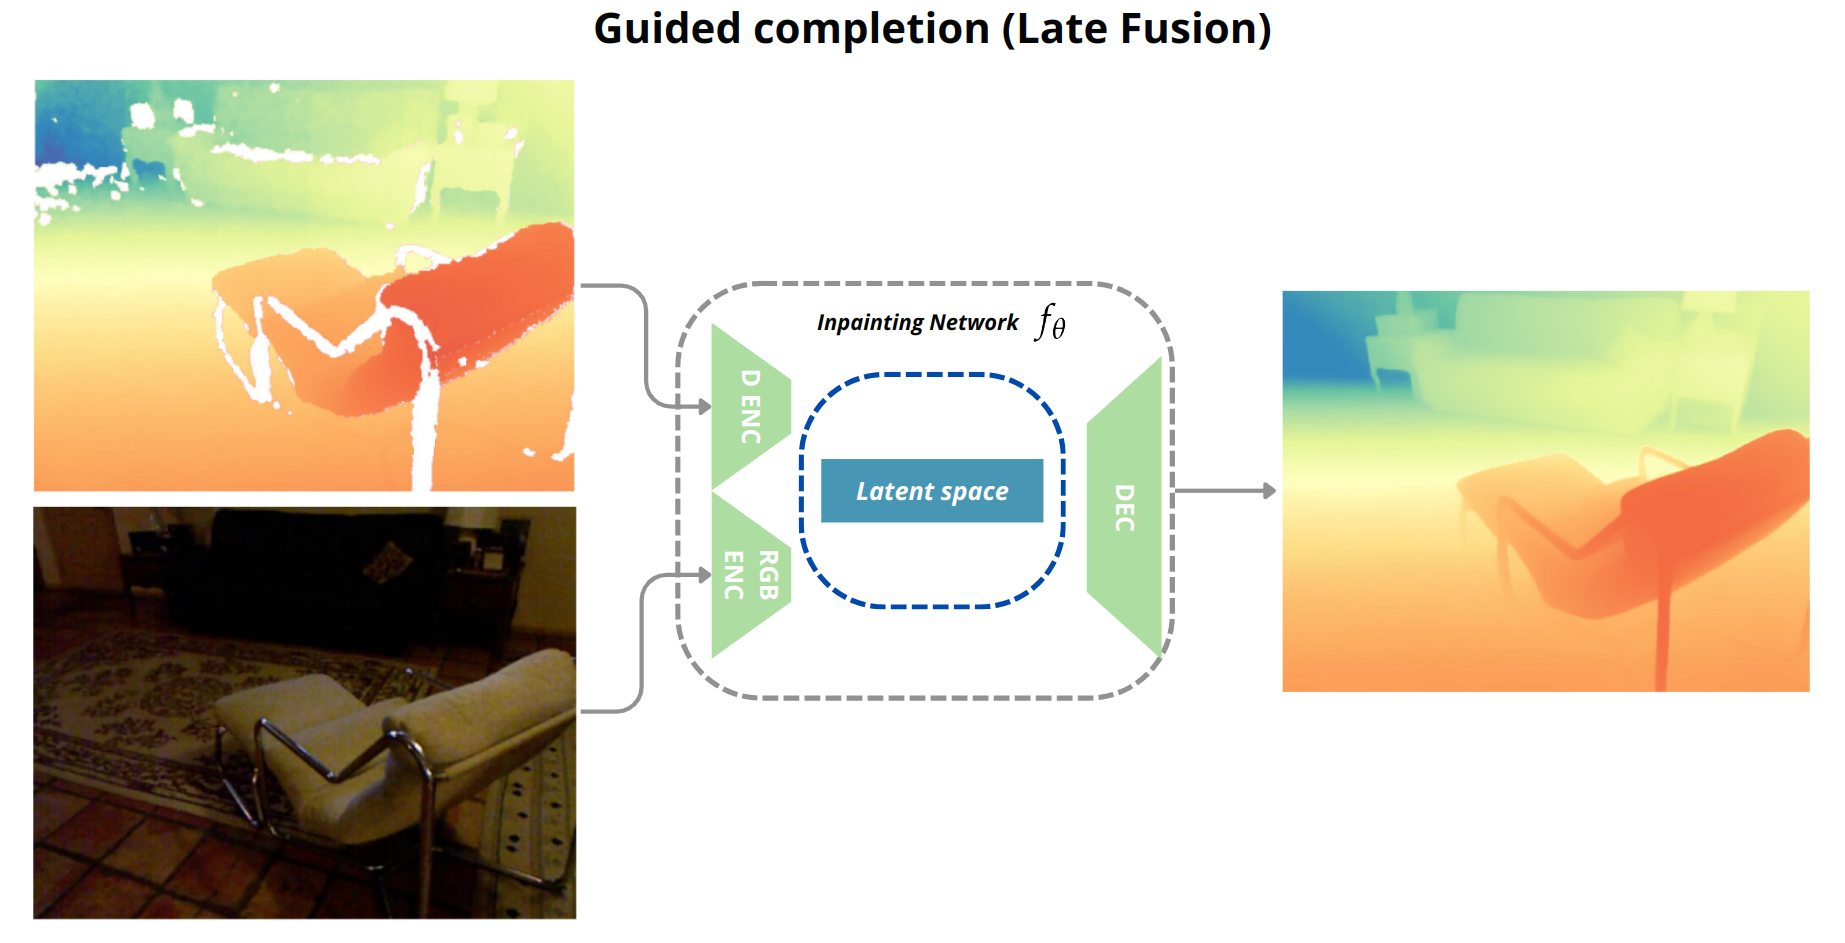
\includegraphics[width=\textwidth]{fig/latefusion.png}
    \caption{Esquema de correção guiada com \textit{Late Fusion}.}
    \label{late}
\end{figure}


\subsection{Large Mask Inpainting}

%Image inpainting is the process of completing or recovering the missing region in the image or removing some objects added to it. 

\textit{Image Inpainting} refere-se ao processo de recuperar regiões faltantes de uma imagem a partir de informação já existente \cite{elharrouss2020image}. Para sintetizar as partes indicadas, é necessário que haja o aprendizado da estrutura global da imagem, sendo imprescindível um vasto campo receptivo na rede neural. Dessa forma, é proposto por \cite{suvorov2022resolution} o sistema LaMa, \textit{Large Mask Inpainting} (Figura \ref{lama}), que é composto por elementos capazes de explorar o campo receptivo apropriado para essa tarefa, sendo eles: i) convoluções rápidas de Fourier (do inglês, \textit{Fast Fourier Convolutions}), ii) o uso de perda perceptual baseada em uma rede de segmentação e iii) uma estratégia de geração de máscaras para treinamento de alta cobertura.

\begin{figure}[h]
    \centering
    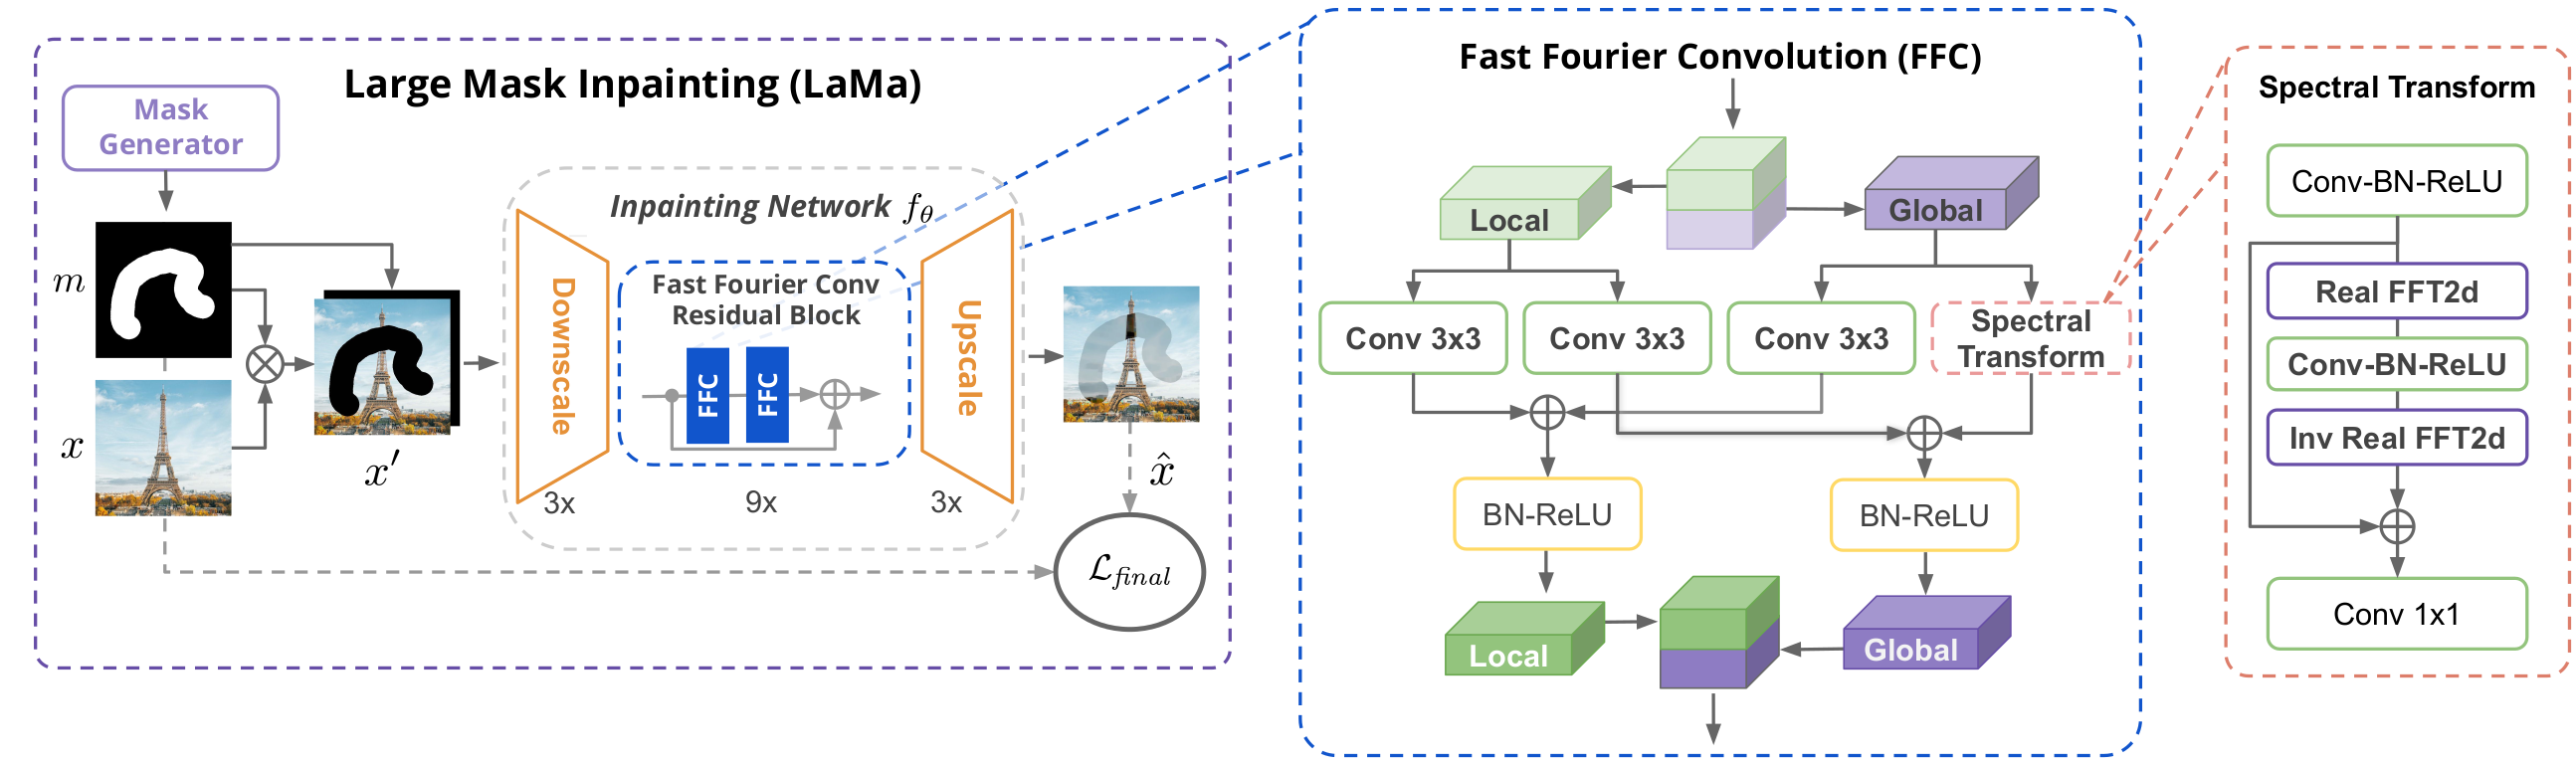
\includegraphics[width=\textwidth]{fig/lama.png}
    \caption{Esquema do método LaMa \cite{suvorov2022resolution}.}
    \label{lama}
\end{figure}

%explain receptive field?




\section{Análise com Aplicação}


\section{Considerações Metodológicas}

